\section{Auxiliary Definitions}\label{subsec:auxdefs}
In this section, we present the auxiliary definitions used in our formalization in 
Figure~\ref{fig:auxfunc}. To begin with, we
introduce the basic functions: $\ext, \overrideSet$ and $\prune$. $\ext(I, J)$
simply indicates that interface $I$ directly extends interface $J$. 
$\overrideSet(I, J)$ returns a set of methods defined in $I$ that have ``$\kwoverride \; J$''
in their signatures. Notice that $\overrideSet(I, I)$ is a special representative of
the ``originally-defined'' method set from $I$. The $\prune$ function takes a set of
types, and filters out those that have subtypes in the same set. Finally in the returned set,
none of them has a subtyping to one another, since all super types have been removed.


% $\begin{array}{l}
% \InTextDef{15ex}{
% \mBody(\m,\C_0)
% }{
% \override(\methods(\m),
% \tops(\m,\Cs))
% }\\
% \InTextWith{\metaVar{IT}(\C_0) =
% \ \ann\ \QM{interface}\ \C_0\ \QM{extends}\ \C_1\ldots\C_n}\\
% \hspace{1.2in}\oC\methods\ \cC \mbox{ and } \C\in\Cs \mbox{ if } \C_i\subtype\C, i\in 1..n

% \end{array}$

% \noindent The definition of $\mBody$ reconstructs the full set of supertypes $\Cs$ and then delegates the work to two other auxiliary functions:
%  $\tops(m,\Cs)$ and $\override(\method,\methods)$.


\begin{figure*}[t]
    \begin{mathpar}
    \inferrule* [left=]
        {  \mostSpecific(m, I_d, I_s) = \{I\} \\
            \mostSpecificOverride(m, I_d, I) = \{J\} \\
            \kwinterface \; J \; \kwextends \; \overline{J} \; \{\method{I_e}{m}{I_x}{x}{I}{e_0}\ldots\}}
        {\mbody(m, I_d, I_s) = (J, \overline{I_x} \; \overline{x}, I_e \; e_0)}
    
    \inferrule* [left=]
        {  \mostSpecific(m, I_d, I_s) = \{I\} \\
            \mostSpecificOverride(m, I_d, I) = \{J\} \\
            \kwinterface \; J \; \kwextends \; \overline{J} \; \{\absmethod{I_e}{m}{I_x}{x}{I}\}}
        {\mbody(m, I_d, I_s) = (J, \overline{I_x} \; \overline{x}, I_e \; \o)}
    
    \inferrule* [left=]
    { originalIntfs = \; \{K \mid \subt{I}{K}, \; \subt{K}{J} \; \lor \; \subt{J}{K}, \; $and$\; m \in \overrideSet(K, K) \} }
    {\mostSpecific(m, I, J) = \prune(originalIntfs) }

    
    \inferrule* [left=]
        { overrideIntfs = \; \{ K\mid I <: K, \; K <: J\; $and$ \;
            m \in \overrideSet(K, J)  \} }
        {\mostSpecificOverride(m, I, J) = \prune(overrideIntfs)}
    
    \prune(set) = \{I \in set \; | \; \nexists J \in set\setminus I, J <: I\}
    
    % \inferrule* [left=]
    % {   \interface{I}{I}{M}
    %     \\ J \in \overline{I} }
    % {\ext(I, J) \marco{Is this ever used?} \yanlin{Previously used, new version not used.}}
    
    \inferrule* [left=]
    {   \kwinterface \; I \; \kwextends \; \overline{I} \; \{ I_e \; m(\overline{I_x} \; \overline{x}) \;
        \kwoverride \; J \ldots \} }
    {m \in \overrideSet(I, J)}
    
      \inferrule* [left=]
    {   \kwinterface \; I \; \kwextends \; \overline{I} \; \{ I_e \; m(\overline{I_x} \; \overline{x}) \;
        	\kwoverride \; I \ldots \} \\
        \kwinterface \; J \; \kwextends \; \overline{J} \; \{ I_e \; m(\overline{I_x} \; \overline{y}) \;
      	    \kwoverride \; J \ldots \} \\
    }
    {\canOverride(m, I, J)}
    \end{mathpar}
    \caption{Auxiliary functions.}\label{fig:auxfunc}
\end{figure*}

\begin{figure*}[t]
    \centering
    \vspace{-1ex}
    \begin{tabular}{ccc}
        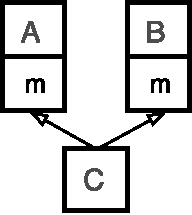
\includegraphics[width=1.5cm]{pics/P1.pdf}\hspace{4pt} &
        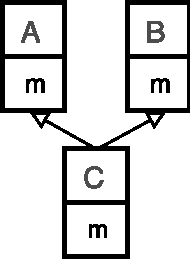
\includegraphics[width=1.5cm]{pics/P2.pdf}\hspace{4pt} &
        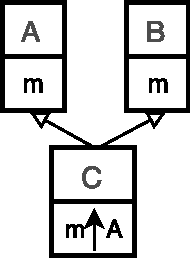
\includegraphics[width=1.5cm]{pics/P3.pdf}\hspace{4pt} \\
        (a) $\mbody(m,C,A) = (A,...)$\ \ \  & (b) $\mbody(m,C,A) = (C,...)$\ \ \  & (c) $\mbody(m,C,A) = (C,...)$
    \end{tabular} \\
   \begin{tabular}{cc}
    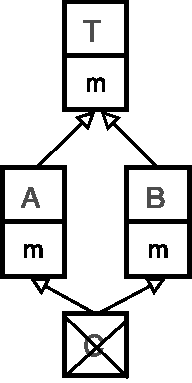
\includegraphics[height=3cm]{pics/P4.pdf}\hspace{4pt} &
    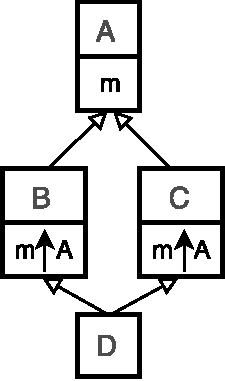
\includegraphics[height=3cm]{pics/P5.pdf}\hspace{4pt} \\ 
    (d) $\mbody(m,D,A) = \keyword{undefined}$\ \ \  & (e) $\mbody(m,D,A) = \keyword{undefined}$
   \end{tabular}
    \caption{Examples on $\mbody$. ``$\uparrow$'' stands for hierarchical overriding.}\label{fig:examplesmbody}
    %\saveSpaceFig
\end{figure*}

\subsection{$\mostSpecific$ and $\mostSpecificOverride$}

$\mostSpecific$ is an auxiliary function that finds the most specific original implementations of a method. Let us consider $\mostSpecific(m, I, J)$, what it returns is a set of interfaces, each including its own $m$ as a most specific implementation. Such a set may contain several elements, but that implies ambiguity; what we expect is actually a singleton set. By the definition of $\mostSpecific$ shown in Figure~\ref{fig:auxfunc}, an interface belongs to the return set if and only if:
\begin{itemize}
    \item It has an original definition of $m$;
    \item It is a supertype of $I$;
    \item It is along path $J$, meaning that it is either a supertype or a subtype of $J$ (including $J$ itself);
    \item It does not have a subtype in the same set because we have used $prune$ to filter out all super types.
\end{itemize}
We could have put $set1$ and $set2$ together, but the current
definition is clearer.

The $\mostSpecific$ function only focuses on original method implementations, all the hierarchical overriding methods are omitted during that time. On the other hand, another auxiliary function $\mostSpecificOverride(m, I, J)$ has the assumption that $J$ defines an original $m$, and this function tries to find the most specific implementations that hierarchically overrides such an $m$. Just as $\mostSpecific$, $\mostSpecificOverride$ also returns the set of interfaces after pruning. An interface belongs to the return set if and only if:
\begin{itemize}
    \item It is between $I$ and $J$;
    \item It hierarchically overrides $J.m$;
    \item It does not have a subtype in the same set.
\end{itemize}
The algorithm for finding the most specific hierarchical overriding method is quite similar to that for finding the most specific original method. A hierarchical overriding is not allowed to work on another hierarchical overriding, and one can hide another if their interfaces have subtyping relations. If they do not hide each other, the result implies ambiguity.


\subsection{$\canInstantiate$}
We use the auxilary function $\canInstantiate(I)$ to check whether an interface $I$ can be instantiated or not.
The algorithm is decribed below:

$$\forall m, \forall J \in \mostSpecific(m, I, I), $$
\begin{enumerate}
\item For any $m$, suppose $\mostSpecific(m, I, I) = \overline{J}$, where $\overline{J}$ is a list of interfaces.
\item If $\forall J_i \in \overline{J}, if \mostSpecificOverride(m, I, J_i) = \{ K \} $ and $m$ in $K$ is not abstract, 
then $\canInstantiate(I) = true$, else $\canInstantiate(I) = false$.
\end{enumerate}

\begin{comment}
\subsection{$\mbodyStatic$}
The auxilary function $\mbodyStatic$ serves for method loopup for static method invocation. 
The brief description of the algorithm follows:
\begin{mathpar}
    \inferrule* [left=]
        {  %\mostSpecific(m, I, I) = \{J\} \\
            \kwinterface \; J \; \kwextends \; \overline{J} \; \{\method{I_e}{m}{I_x}{x}{J'}{e_0}\ldots\}}
        {\mbodyStatic(m, J, J') = (J, \overline{I_x} \; \overline{x}, I_e \; e_0)}

    \inferrule* [left=]
        {  %\mostSpecific(m, I, I) = \{J\} \\
            \kwinterface \; J \; \kwextends \; \overline{J} \; \{\absmethod{I_e}{m}{I_x}{x}{J'}\ldots\}}
        {\mbodyStatic(m, J, J') = (J, \overline{I_x} \; \overline{x}, I_e \; \o)}
\end{mathpar}    
\end{comment}

\subsection{$\mbody$ and $\mtype$}

$\mbody(m, I_d, I_s)$, as defined in Figure~\ref{fig:auxfunc}, denotes a method body lookup function.
We use $I_d, I_s$, since $\mbody$ is usually invoked by a receiver of a method $m$, with its dynamic
type $I_d$ and static type $I_s$. Such a function returns the most specific method implementation, more
accurately, its parameters, returned expression and the types. It considers both originally defined methods and hierarchical overriding methods, so $\mostSpecific$ and $\mostSpecificOverride$ are invoked.

To calculate $\mbody(m, I_d, I_s)$:
\begin{itemize}
    \item First, it invokes $\mostSpecific(m, I_d, I_s)$ and returns a set.
    \item If $\mostSpecific$ returns a singleton set $\{I\}$, then it is good, otherwise, $\mbody$ is undefined in
    this case. The set $\{I\}$ implies that we will use the $m$ from $I$ without ambiguity. Moreover, we have to invoke $\mostSpecificOverride(m, I_d, I)$, to check if there are updated versions of $m$ between $I_d$ and $I$. Again we forbid ambiguity, so the expected set after pruning is also a singleton set $\{J\}$.
    \item Finally, we fetch the implementation of $m$ in interface $J$ and return its related information.
\end{itemize}
The definition of $\mtype$ used in typing rules simply relies on $\mbody$. In short,
$$\mbody(m, I, I) = (J, \overline{I_x}\ \overline{x}, I_e\ ?) \ \Longrightarrow\ \mtype(m, I) = \overline{I_x}\rightarrow I_e$$

\begin{comment}
$mbody(m, I)$ algorithm:
\begin{itemize}
    \item If m is defined in I directly, then return I.m()
    \item Else, let $\overline{I'} = mdefined(fathers(I))$, all ancestors of $I$ that has directly defined $m()$.
    \item $\overline{I''} = needed(\overline{I'})$, keep only interfaces that are needed, which are not super-interface of others.
    \item If $\overline{I''}$ is unique, then return this unique one. Else if any two I1,I2 in $\overline{I''}$ share a parent in $\overline{I'}$, then diamond conflict is detected, report error. Else return multiple $m()$s.
\end{itemize}
\end{comment}

\begin{comment}
\subsubsection{\collectMethods}
\[ \collectMethods(I) = \left( \bigcup_{I_i \in \overline{I}} \methods(I_i) \right) \bigcup \methods(I) \]
\[ \methods(I) = \overline{M}, \text{where } IT(I) = \interface{I}{I}{M} \]
\end{comment}

\subsection{Examples}

Examples for $\mbody$ are shown in Figure~\ref{fig:examplesmbody}. Note that we use \lstinline|m| to denote an original method, and ``\lstinline|m|$\uparrow$\lstinline|A|'' for hierarchical overriding on \lstinline|A|. For each small example, the result
gives the interface to which $m$ is dispatched. (a) is a basic model for unintentional method conflicts; (b) and (c) demonstrate
that hierarchical dispatch can find the most specific original method and hierarchical overriding method. More interesting are the two bad examples
(d) and (e), they both fail on $\mbody$. (d) is the well-known diamond inheritance, which our model also forbids, and (e) is similar to
(d) because the two hierarchical overriding methods are working on the same operation. Both counter-examples imply that \lstinline|new D().A::m()| will
lead to ambiguity, and in order for type soundness, both have to be denied by the type checker. This is guaranteed by the interface check
\textsc{(T-Intf)} in Figure~\ref{fig:typingrules}.